\documentclass{article}
\usepackage{amsthm}
\usepackage{amsmath}
\usepackage{etoc}
\usepackage{amssymb}
\usepackage{enumitem}
\usepackage{apacite}
\usepackage{mathtools, amssymb}
\usepackage{bm}
\usepackage{tikz}
\usepackage{fancyhdr}
\usepackage{caption}
\usepackage{tabto}
\usepackage{hyperref}
\usepackage{graphicx}
\usepackage[nottoc]{tocbibind}
\usepackage{calrsfs}
\usepackage{changepage}
\usepackage{siunitx}
\usepackage{listings}% http://ctan.org/pkg/listings
\lstset{
  basicstyle=\ttfamily,
  mathescape
}
\usetikzlibrary{arrows.meta, automata, positioning, quotes}



% Margins
\usepackage[top=2.5cm, left=3cm, right=3cm, bottom=4.0cm]{geometry}
% Colour table cells

% Get larger line spacing in table
\newcommand{\tablespace}{\\[1.25mm]}
\newcommand\Tstrut{\rule{0pt}{2.6ex}}         % = `top' strut
\newcommand\tstrut{\rule{0pt}{2.0ex}}         % = `top' strut
\newcommand\Bstrut{\rule[-0.9ex]{0pt}{0pt}}   % = `bottom' strut

%%%%%%%%%%%%%%%%%
%     Title     %
%%%%%%%%%%%%%%%%%
\title{Theory of automata and Formal languages}
\author{Fernando Javier López Cerezo \\ Practice 3}
\date{\today}

\begin{document}
\maketitle

\section*{Problem 1}
In exercise 1 we are asked to define a TM that computes the addition of two numbers. This is my proposal: \\ 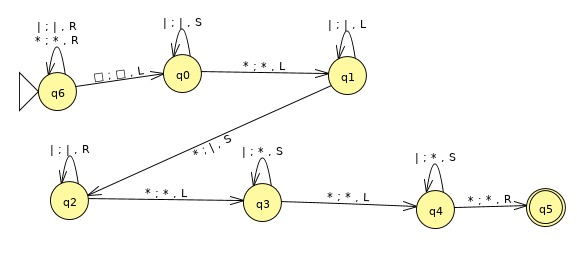
\includegraphics[width=\linewidth]{TM.png} 

\section*{Problem 2}
In exercise 2 we are asked to define a recursive function for the sum of three values. My proposal is addition3 $= \langle\langle\pi^1_1|\sigma(\pi^3_3)\rangle|\sigma(\pi^4_4)\rangle$. We can check it works in the following example: \\ 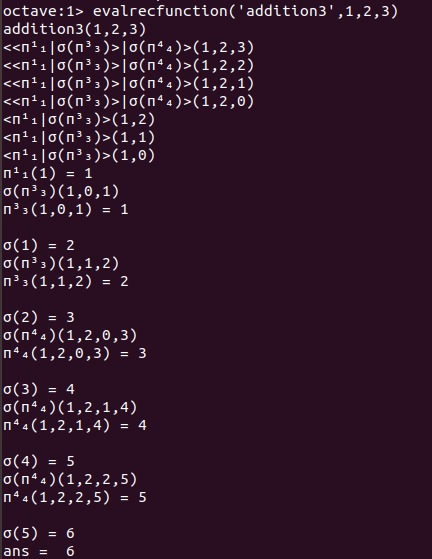
\includegraphics[width=\linewidth]{add.png} 

\section*{3}
Exercise 3 asks us to write a WHILE program that computes the sum of three numbers. My proposal is the following: \begin{lstlisting}
Sum3=(3,s)
s:
   while X2 $\neq$  0 do
      X1 := X1 + 1
      X2 := X2 - 1;
   od
   
   while X3 $\neq$  0 do
      X1 := X1 + 1
      X3 := X3 - 1;
   od
    
	


\end{lstlisting}

%%%%%%%%%%%%%%%%%
%   Problem 1   %
%%%%%%%%%%%%%%%%%

\end{document}